% ============================================================
% 第2章：函数的图像——从代数到几何的翻译
% ============================================================

\chapter{函数的图像——从代数到几何的翻译}

\begin{applicationbox}
\textbf{学完本章你能做什么？}
\begin{enumerate}
  \item \textbf{学之前}：你理解了函数是"输入$\to$规则$\to$输出"，但只能在纸上算数。
  \item \textbf{学之后}：你能把任何一个函数\textbf{画成图像}，也能从图像上\textbf{读出}它的定义域、值域、零点、单调性——你会用两只眼睛看数学了。
  \item \textbf{日常例子}：心电图就是心脏电信号随时间变化的函数图像。医生不看数字表格，而是看图像的波形——高高低低、节奏快慢——一眼就知道心脏有没有问题。这就是图像的力量。
\end{enumerate}
\end{applicationbox}


% ============================================================
\section{从第1章来——有了函数，为什么还要画图？}
% ============================================================

第1章我们学了函数的三要素：定义域、对应法则、值域。

这些东西用公式表达很精确，但有一个问题：\textbf{不直观}。

\begin{center}
\fcolorbox{blue!40}{blue!5}{\parbox{0.85\textwidth}{
\textbf{对比：} \\
公式 \(f(x) = x^2\) —— 你看到它，需要想一下才知道"这是一个开口向上的抛物线"。\\
图像 \(y = x^2\) 的图 —— 你一眼就看到它的形状、对称性、最低点在(0,0)。
}}
\end{center}

画函数图像就是把\textbf{抽象的代数关系翻译成直观的几何图形}。\\
这是数学中最重要的思想之一——\textbf{数形结合}。

\begin{notebox}
\textbf{数形结合}（读作 shù xíng jié hé）：\\
代数和几何不是两门独立的学科，而是同一个数学事实的两种语言。\\
函数是连接这两种语言的桥梁。
\end{notebox}


% ============================================================
\section{平面直角坐标系回顾}
% ============================================================

在画函数图像之前，先快速回顾坐标系。

\begin{definitionbox}[平面直角坐标系]
\begin{itemize}
  \item \textbf{\(x\) 轴}（横轴）：水平的数轴，向右为正
  \item \textbf{\(y\) 轴}（纵轴）：垂直的数轴，向上为正
  \item \textbf{原点 \(O\)}：两条轴的交点，坐标为 \((0,0)\)
  \item \textbf{坐标 \((x, y)\)}：先横后纵，确定平面上唯一一个点
\end{itemize}
\end{definitionbox}

函数 \(y = f(x)\) 的图像，就是所有满足 \(y = f(x)\) 的点 \((x, y)\) 的集合。

用数学语言说：
\[
\text{函数 } f \text{ 的图像} = \{\, (x, f(x)) \mid x \in D \,\}
\]
其中 \(D\) 是定义域。


% ============================================================
\section{描点法——最根本的画图方法}
% ============================================================

画任何函数图像，最根本的方法就是\textbf{描点法}。\\
虽然是"笨办法"，但它是理解函数图像的起点。

\subsection{描点法的三个步骤}

\begin{definitionbox}[描点法画函数图像]
\textbf{第1步：列表}——选择一些有代表性的 \(x\) 值，算出对应的 \(f(x)\)。\\
\textbf{第2步：描点}——在坐标系中画出每个 \((x, f(x))\)。\\
\textbf{第3步：连线}——用平滑的曲线按 \(x\) 从小到大的顺序连接各点。
\end{definitionbox}

\subsection{用描点法画 \(y = x^2\)}

\begin{examplebox}[1]
用描点法画 \(y = x^2\) 的图像。

\textbf{第1步：列表}

\begin{center}
\begin{tabular}{c|c|c|c|c|c|c|c}
\(x\) & -3 & -2 & -1 & 0 & 1 & 2 & 3 \\
\hline
\(y = x^2\) & 9 & 4 & 1 & 0 & 1 & 4 & 9 \\
\end{tabular}
\end{center}

\textbf{第2步：描点}
在坐标系中画出 \((-3,9)\)、\((-2,4)\)、\((-1,1)\)、\((0,0)\)、\((1,1)\)、\((2,4)\)、\((3,9)\)。

\textbf{第3步：连线}
按 \(x\) 从小到大的顺序，用平滑曲线连接各点。

\begin{center}
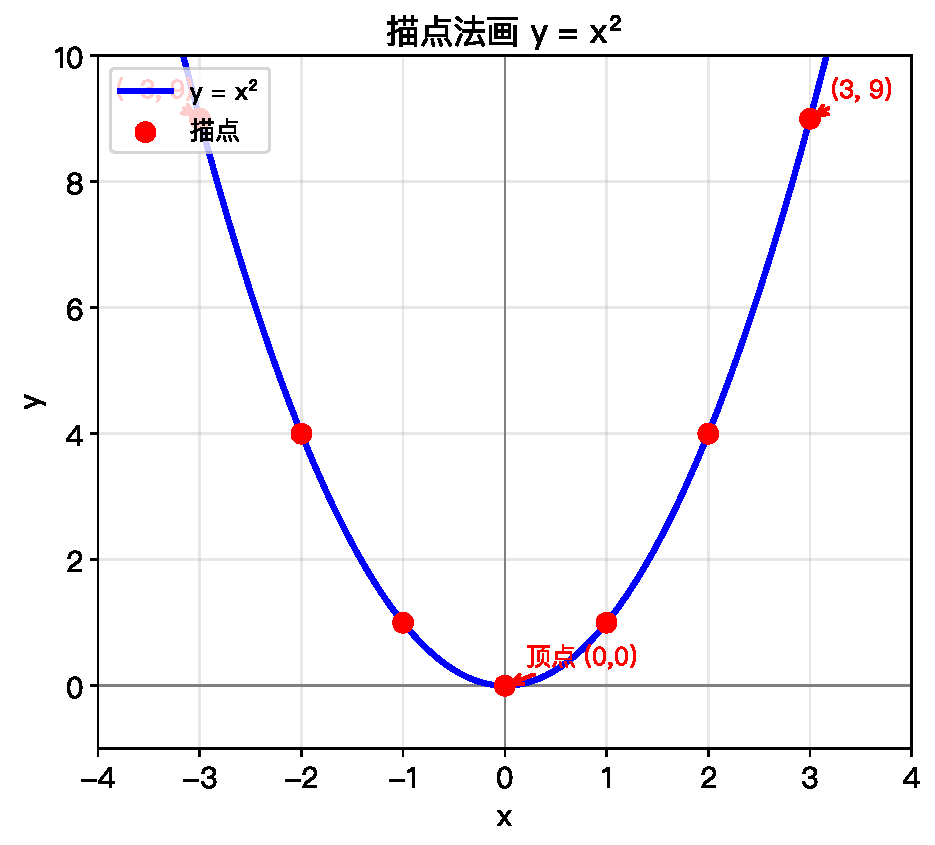
\includegraphics[width=0.55\textwidth]{figures/ch02_sketch_x2.pdf}
\end{center}

你看，这些点排成一条\textbf{抛物线}的形状。

\textbf{从图像能看出什么？}
\begin{itemize}
  \item 最低点在 \((0,0)\)——这是最小值点
  \item 关于 \(y\) 轴对称——左边和右边是对称的
  \item 越往两边走，函数值增长越快
\end{itemize}
\end{examplebox}

\begin{examplebox}[2]
用描点法画 \(y = \dfrac{1}{x}\) 的图像。

\textbf{第1步：列表}

\begin{center}
\begin{tabular}{c|c|c|c|c|c|c}
\(x\) & -3 & -2 & -1 & 1 & 2 & 3 \\
\hline
\(y = 1/x\) & -1/3 & -1/2 & -1 & 1 & 1/2 & 1/3 \\
\end{tabular}
\end{center}

注意：\(x = 0\) 不在定义域内，所以表格中没有 \(x = 0\)。

\textbf{第2步：描点，第3步：连线}

\begin{center}
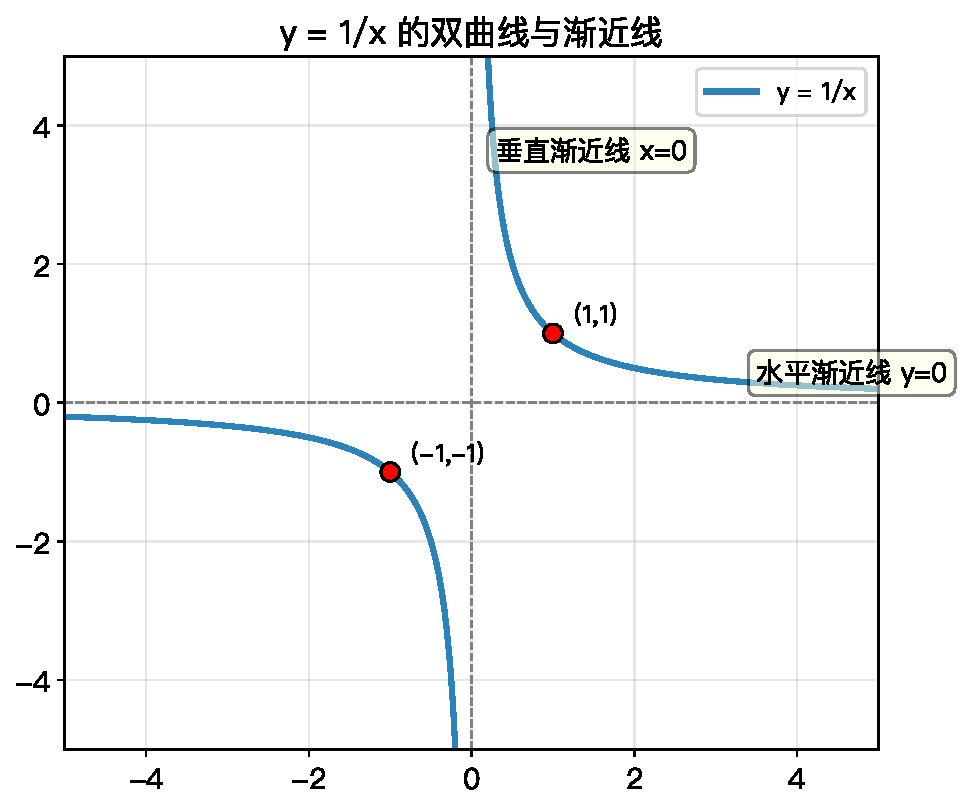
\includegraphics[width=0.5\textwidth]{figures/ch02_reciprocal.pdf}
\end{center}

这个图像叫\textbf{双曲线}（读作 shuāng qū xiàn），它有两条\textbf{渐近线}：
\begin{itemize}
  \item \(x = 0\)（\(y\) 轴）——垂直渐近线，函数在 \(x=0\) 处无定义
  \item \(y = 0\)（\(x\) 轴）——水平渐近线，当 \(x\) 趋向无穷大时函数值趋近 0
\end{itemize}
\end{examplebox}


% ============================================================
\section{六种基本初等函数的图像}
% ============================================================

高中数学中最基本的六种函数，它们的图像必须\textbf{一眼就能认出来}。

\begin{center}
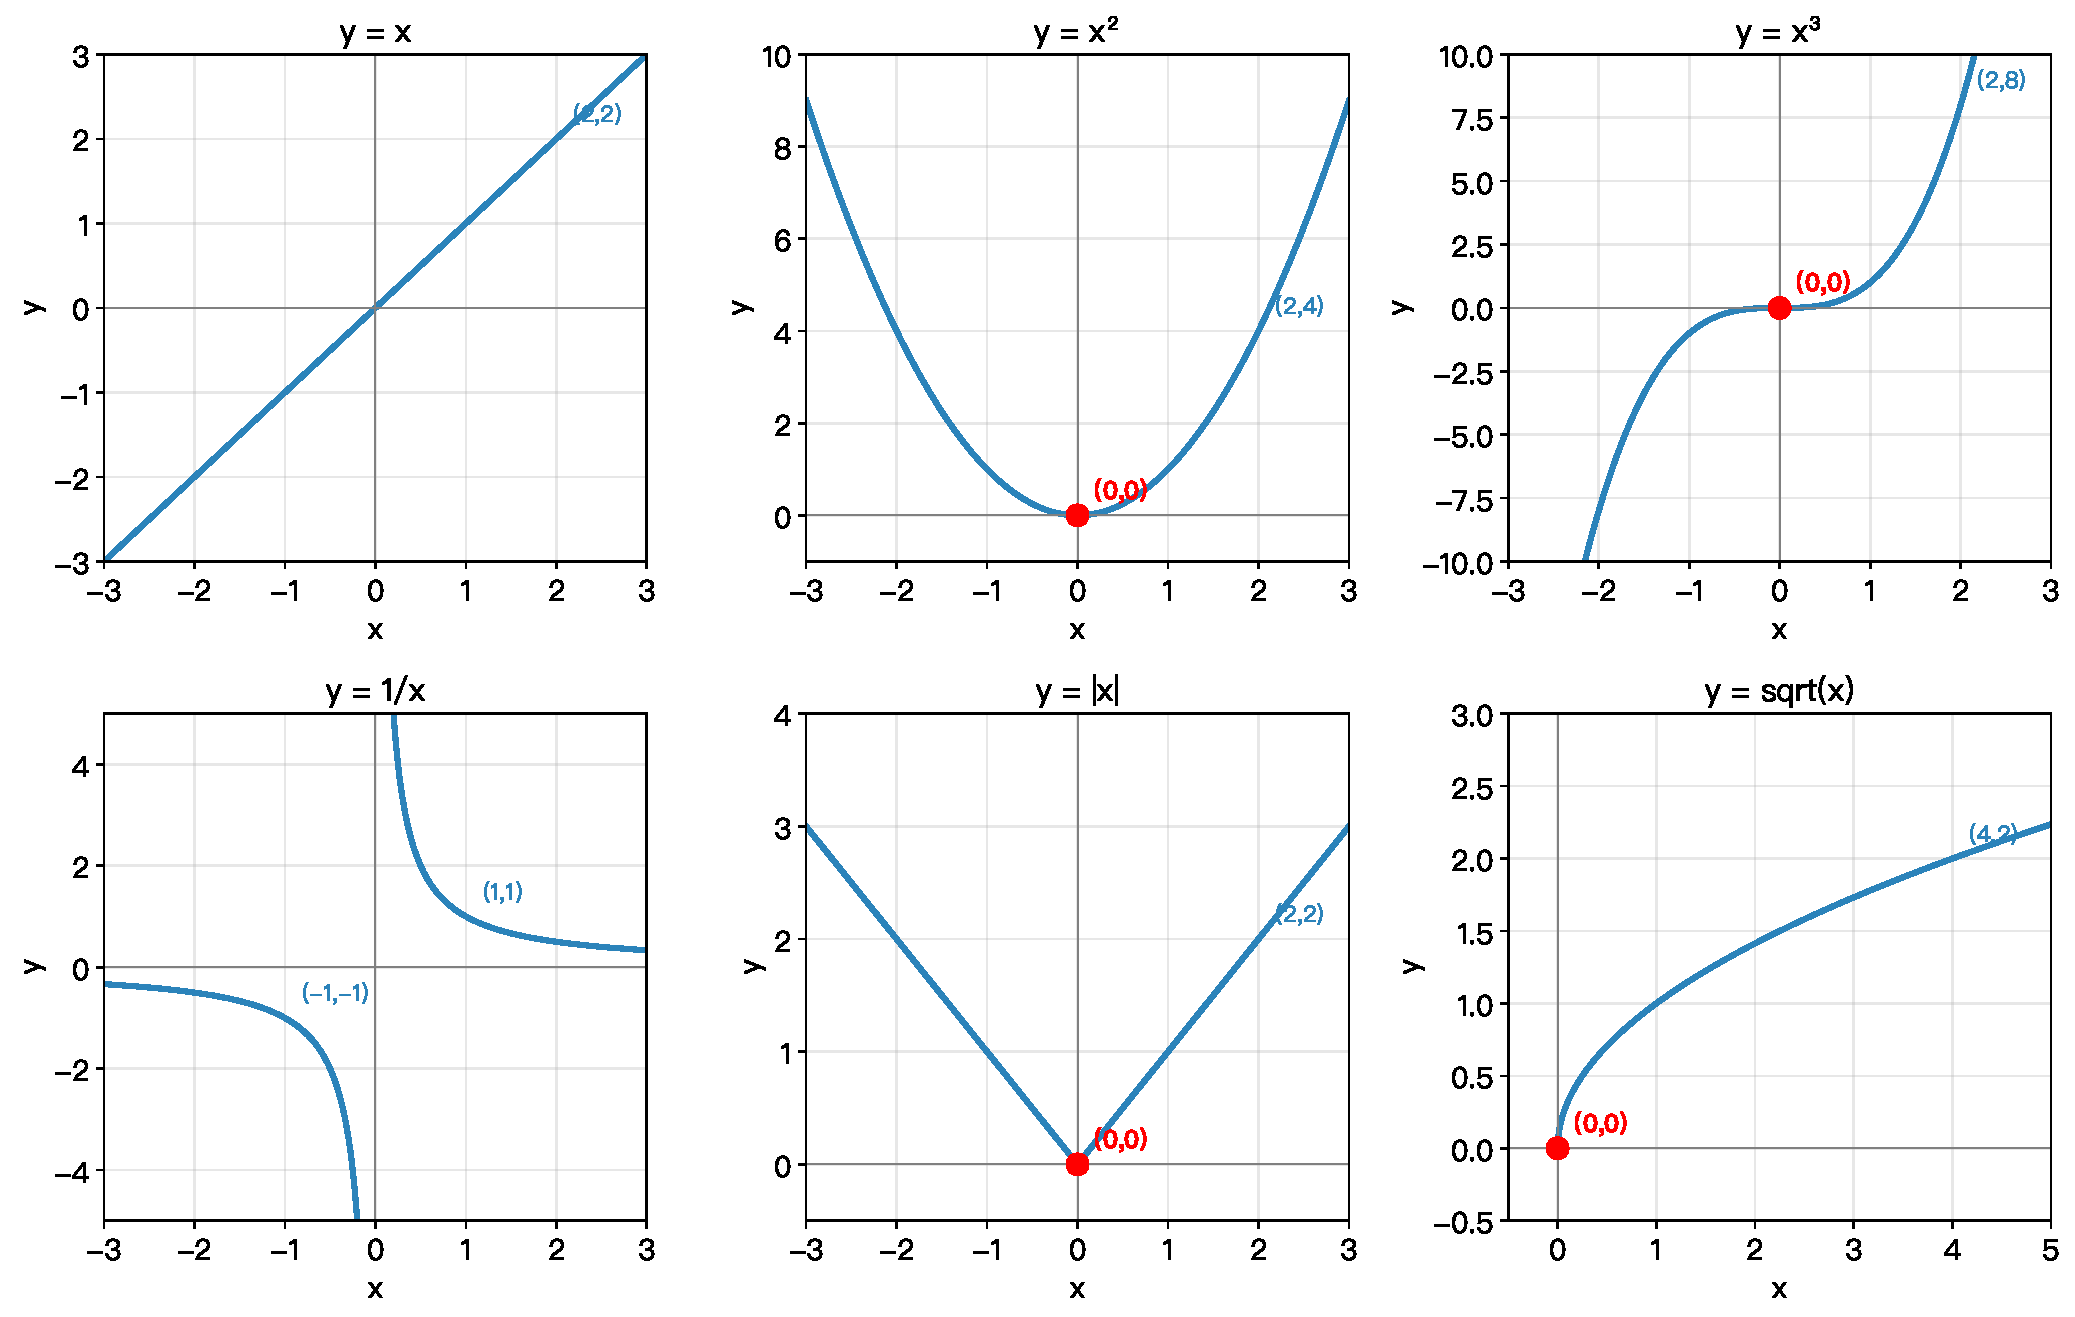
\includegraphics[width=\textwidth]{figures/ch02_six_basic_funcs.pdf}
\end{center}

\begin{examplebox}[3——看图识函数]
对照上图，记住每个函数图像的关键特征：
\begin{enumerate}
  \item \textbf{\(y = x\)}（正比例函数）：通过原点的直线，与 \(x\) 轴成 45° 角
  \item \textbf{\(y = x^2\)}（二次函数）：开口向上的抛物线，顶点在原点
  \item \textbf{\(y = x^3\)}（三次函数）：从左下到右上穿过原点，关于原点对称
  \item \textbf{\(y = 1/x\)}（反比例函数）：双曲线，两条渐近线是坐标轴
  \item \textbf{\(y = |x|\)}（绝对值函数）：V 形，顶点在原点，左右对称
  \item \textbf{\(y = \sqrt{x}\)}（平方根函数）：从原点出发向右延伸，增长速度越来越慢
\end{enumerate}
\end{examplebox}


% ============================================================
\section{从图像读信息——看图说话}
% ============================================================

图像的价值在于：你能\textbf{直接读出}函数的很多重要性质。

\begin{examplebox}[4]
已知函数 \(f(x) = x^3 - x\) 的图像如下：

\begin{center}
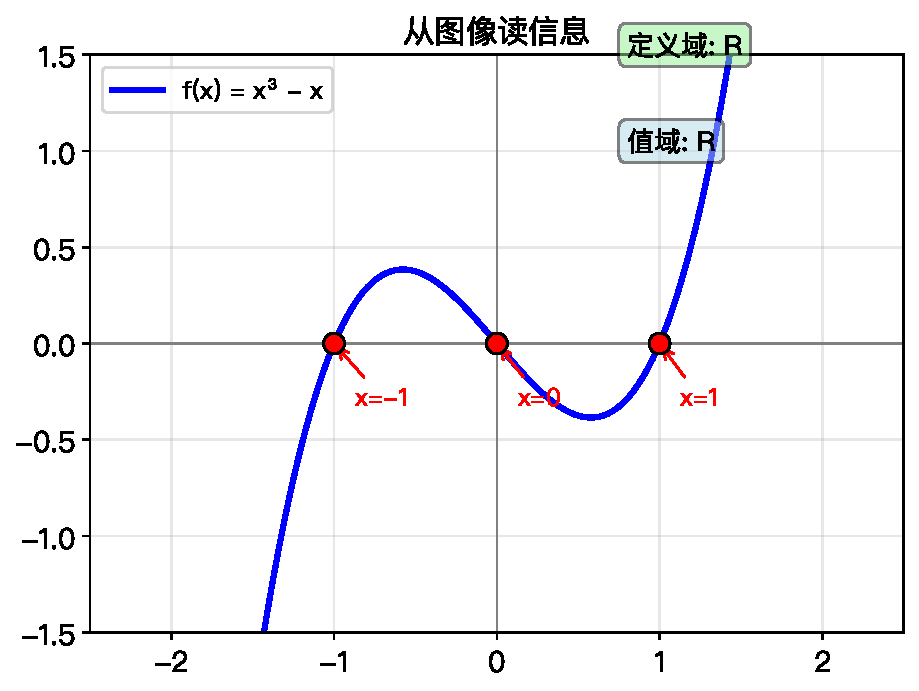
\includegraphics[width=0.5\textwidth]{figures/ch02_read_from_graph.pdf}
\end{center}

从图中可以读出：

\textbf{定义域：} 图像向左右无限延伸 \(\rightarrow\) 定义域为 \(\mathbb{R}\)（全体实数）。

\textbf{值域：} 图像向上下无限延伸 \(\rightarrow\) 值域为 \(\mathbb{R}\)。

\textbf{零点：} 图像与 \(x\) 轴的交点。图中 \(x = -1, 0, 1\) 这三个点处的 \(y = 0\)。\\
验证：\(f(-1) = (-1)^3 - (-1) = -1 + 1 = 0\)，\(f(0) = 0\)，\(f(1) = 1 - 1 = 0\)。

\textbf{单调性：}
\begin{itemize}
  \item 在 \((-\infty, -0.58)\) 上，函数上升（递增）
  \item 在 \((-0.58, 0.58)\) 上，函数下降（递减）
  \item 在 \((0.58, +\infty)\) 上，函数上升（递增）
\end{itemize}
\end{examplebox}

\begin{definitionbox}[从图像读函数性质]
\begin{itemize}
  \item \textbf{定义域}：图像在 \(x\) 轴上的投影范围（看左右到哪）
  \item \textbf{值域}：图像在 \(y\) 轴上的投影范围（看上下到哪）
  \item \textbf{零点}：图像与 \(x\) 轴的交点（\(f(x) = 0\) 的点）
  \item \textbf{单调性}：图像上升 \(\rightarrow\) 递增，图像下降 \(\rightarrow\) 递减
  \item \textbf{最大值/最小值}：图像的最高点/最低点的 \(y\) 坐标
\end{itemize}
\end{definitionbox}


% ============================================================
\section{图像的平移变换——函数搬家}
% ============================================================

在已知一个基本函数图像的基础上，我们可以通过\textbf{平移}得到它的"亲戚"。

\subsection{水平平移：\(y = f(x - a)\)}

\begin{examplebox}[5]
比较 \(y = x^2\) 和 \(y = (x - 2)^2\)：

\begin{center}
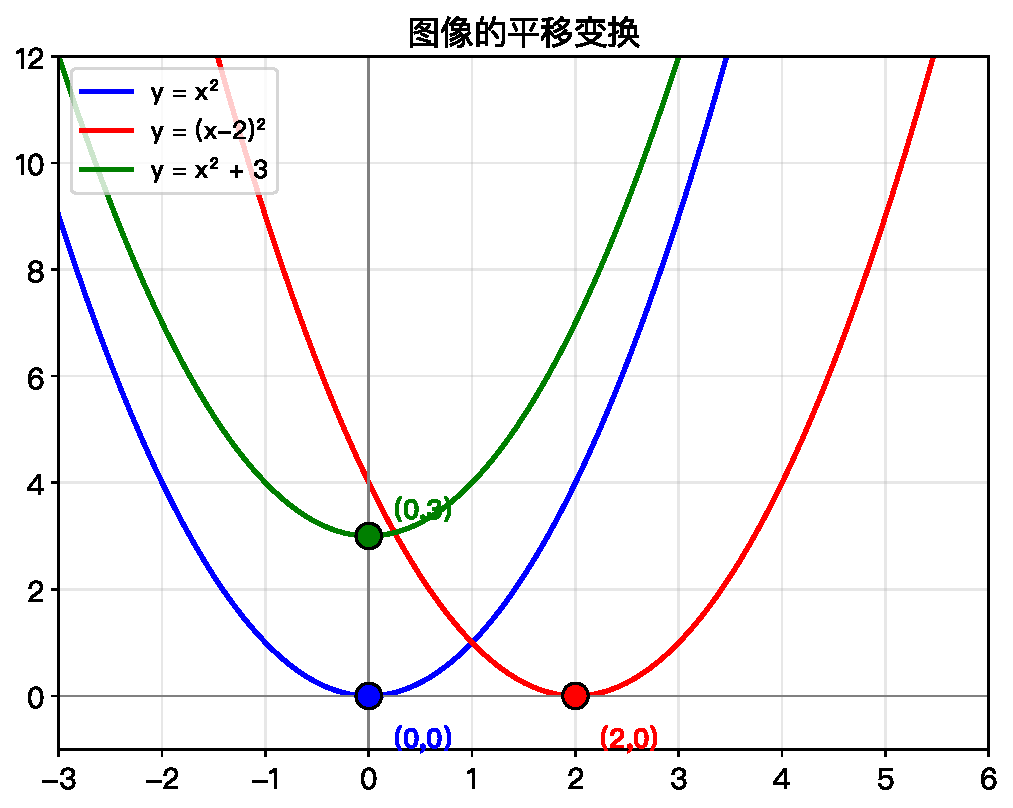
\includegraphics[width=0.55\textwidth]{figures/ch02_translation.pdf}
\end{center}

规律：
\[
y = f(x - a) \text{ 的图像是把 } y = f(x) \text{ 向 \textbf{右} 平移 } a \text{ 个单位}
\]
\[
y = f(x + a) \text{ 的图像是把 } y = f(x) \text{ 向 \textbf{左} 平移 } a \text{ 个单位}
\]

\textbf{注意：} \(x - a\) 是右移，这有点反直觉——因为你想的是"减了 2，应该往左才对"。\\
记忆方法：让 \(x - 2 = 0\) 得 \(x = 2\)，所以顶点从 \(x=0\) 移到了 \(x=2\)——\textbf{右移}。
\end{examplebox}

\subsection{垂直平移：\(y = f(x) + b\)}

容易理解得多：
\[
y = f(x) + b \text{ 的图像是把 } y = f(x) \text{ 向 \textbf{上} 平移 } b \text{ 个单位}
\]
\[
y = f(x) - b \text{ 的图像是把 } y = f(x) \text{ 向 \textbf{下} 平移 } b \text{ 个单位}
\]

\begin{examplebox}[6]
从图中看 \(y = x^2 + 3\)：\\
把 \(y = x^2\) 向上平移 3 个单位，顶点从 \((0,0)\) 移到 \((0,3)\)。
\end{examplebox}


% ============================================================
\section{图像的对称变换——翻转}
% ============================================================

\subsection{关于 \(x\) 轴对称：\(y = -f(x)\)}

\begin{examplebox}[7]
比较 \(y = x^2\) 和 \(y = -x^2\)：

\begin{center}
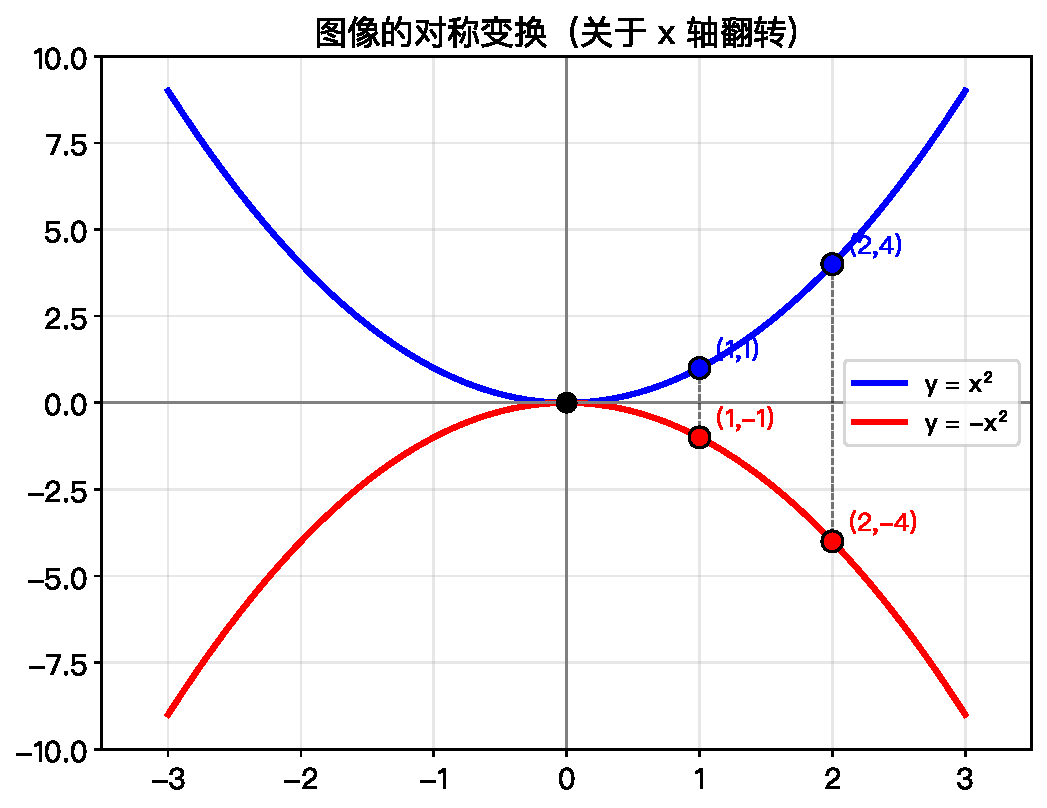
\includegraphics[width=0.55\textwidth]{figures/ch02_symmetry.pdf}
\end{center}

规律：
\[
y = -f(x) \text{ 的图像是把 } y = f(x) \text{ 关于 \(x\) 轴翻转（上下翻转）}
\]

从图中可以看到：\((2, 4)\) 翻到了 \((2, -4)\)，\((1, 1)\) 翻到了 \((1, -1)\)。\\
原来开口向上的抛物线变成了开口向下。
\end{examplebox}

\subsection{关于 \(y\) 轴对称：\(y = f(-x)\)}

\[
y = f(-x) \text{ 的图像是把 } y = f(x) \text{ 关于 \(y\) 轴翻转（左右翻转）}
\]

例：\(y = e^{-x}\) 的图像就是把 \(y = e^x\) 左右翻转（以后学指数函数时会看到）。


% ============================================================
\section{图像的翻折变换——把负的变成正的}
% ============================================================

翻折变换有两种常见形式：

\subsection{\(y = |f(x)|\)——把 \(x\) 轴下方的部分翻到上方}

\begin{examplebox}[8]
比较 \(y = x^2 - 1\) 和 \(y = |x^2 - 1|\)：

\begin{center}
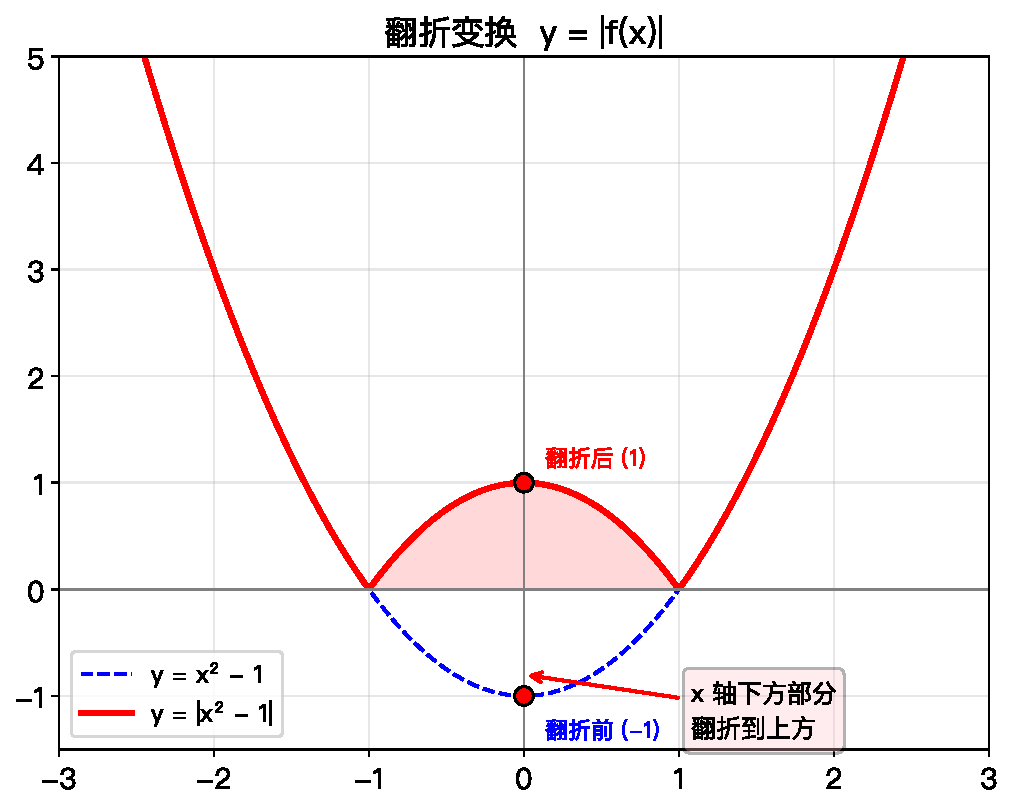
\includegraphics[width=0.55\textwidth]{figures/ch02_abs_flip.pdf}
\end{center}

规律：
\[
y = |f(x)| \text{ 的图像：保留 } y = f(x) \text{ 在 \(x\) 轴上方的部分，}\\
\text{把 \(x\) 轴下方的部分沿 \(x\) 轴翻折到上方}
\]

\textbf{验证：}
\begin{itemize}
  \item \(x = 2\) 时，\(x^2 - 1 = 3\)，\(|3| = 3\)——没变
  \item \(x = 0.5\) 时，\(x^2 - 1 = -0.75\)，\(|-0.75| = 0.75\)——从下方翻到了上方
\end{itemize}
\end{examplebox}

\subsection{\(y = f(|x|)\)——保留右边，对称到左边}

\[
y = f(|x|) \text{ 的图像：保留 } y = f(x) \text{ 在 \(y\) 轴右侧的部分，}\\
\text{去掉左侧部分，把右侧部分关于 \(y\) 轴对称到左侧}
\]


% ============================================================
\section{垂线检验法——判断一个曲线是不是函数}
% ============================================================

\begin{theorembox}[垂线检验法]
在平面上任意画一条竖直线（与 \(y\) 轴平行的直线）：
\begin{itemize}
  \item 如果每条竖直线\textbf{最多}与曲线交于\textbf{一个}点 \(\rightarrow\) 这是\textbf{函数的图像}
  \item 如果某条竖直线与曲线交于\textbf{两个或更多}点 \(\rightarrow\) \textbf{不是函数的图像}
\end{itemize}
\end{theorembox}

\begin{center}
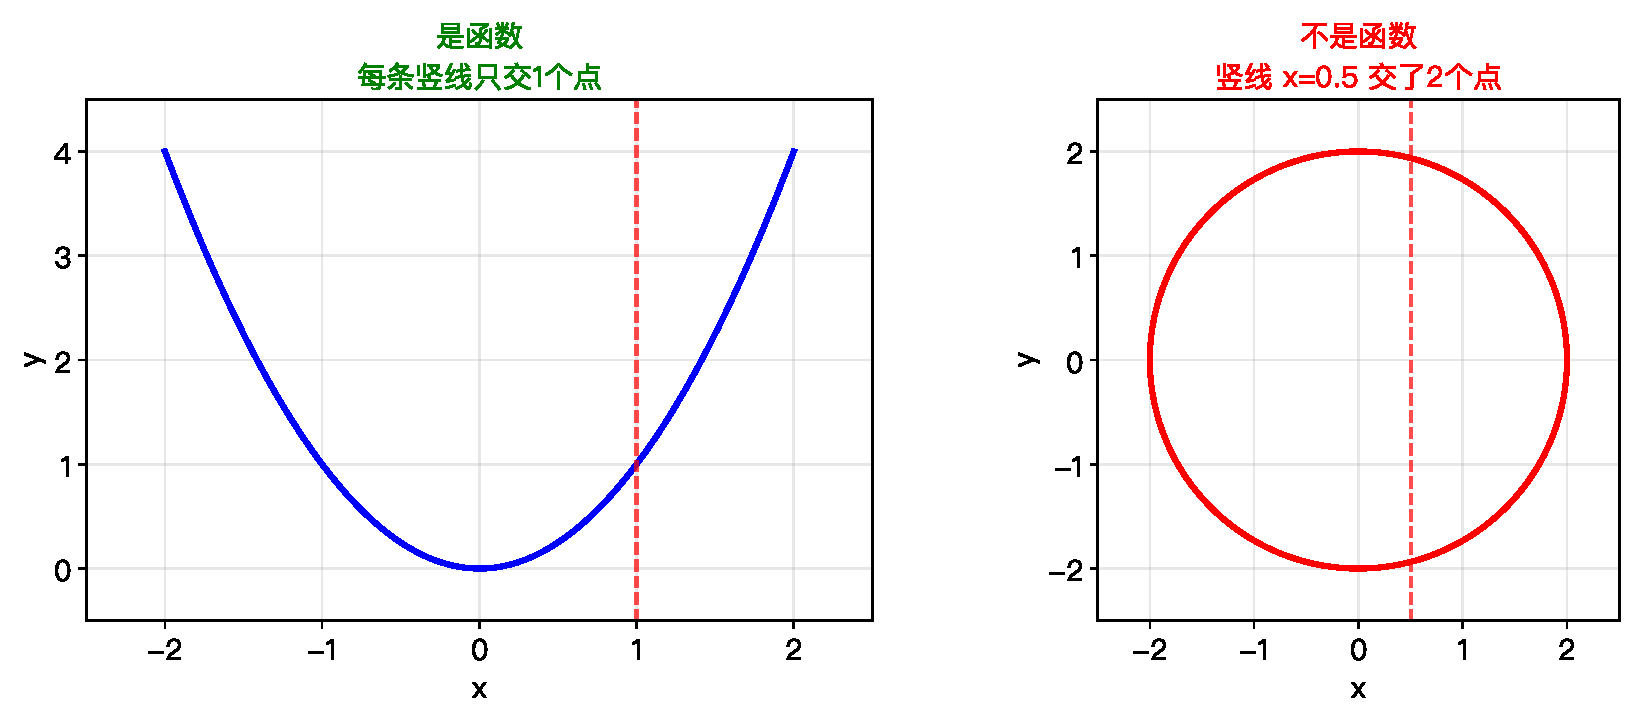
\includegraphics[width=0.75\textwidth]{figures/ch02_vertical_line_test.pdf}
\end{center}

\begin{examplebox}[9]
判断以下曲线是不是函数的图像：
\begin{enumerate}
  \item \textbf{直线 \(y = 2x + 1\)}：任意竖直线只交 1 个点 \(\rightarrow\) 是函数 [OK]
  \item \textbf{圆 \(x^2 + y^2 = 9\)}：竖直线 \(x = 1\) 与圆交于两个点 \(\rightarrow\) 不是函数 [X]
  \item \textbf{抛物线 \(y = x^2\)}：任意竖直线只交 1 个点 \(\rightarrow\) 是函数 [OK]
  \item \textbf{折线 \(y = |x|\)}：任意竖直线只交 1 个点 \(\rightarrow\) 是函数 [OK]
\end{enumerate}
\end{examplebox}


% ============================================================
\section{符号卡片}
% ============================================================

\begin{symbolcard}
\((x, f(x))\) & \verb|(x, f(x))| & 读作"点 x f of x" & 函数图像上的一个点 \\
\(\{\, (x, f(x)) \mid x \in D \,\}\) & \verb+{ (x,f(x)) | x in D }+ & 读作"所有满足...的点" & 函数图像的集合表示 \\
\(y = f(x - a)\) & \verb|y = f(x - a)| & —— & 右移 \(a\) 个单位 \\
\(y = f(x) + b\) & \verb|y = f(x) + b| & —— & 上移 \(b\) 个单位 \\
\(y = -f(x)\) & \verb|y = -f(x)| & —— & 关于 \(x\) 轴对称 \\
\(y = |f(x)|\) & \verb+y = |f(x)|+ & —— & 把 \(x\) 轴下方翻折到上方 \\
\end{symbolcard}


% ============================================================
\section{代码验证}
% ============================================================

\begin{lstlisting}[caption=用 Python 画函数图像]
import numpy as np
import matplotlib.pyplot as plt

# 设置中文字体
plt.rcParams['font.sans-serif'] = ['PingFang SC']
plt.rcParams['axes.unicode_minus'] = False

# 画三个函数在同一坐标系中
x = np.linspace(-4, 4, 400)
plt.figure(figsize=(8, 5))

plt.plot(x, x**2, 'b-', linewidth=2, label='y = x²')
plt.plot(x, x**3, 'r-', linewidth=2, label='y = x³')
plt.plot(x, 2**x, 'g-', linewidth=2, label='y = 2^x')

plt.axhline(0, color='gray', linewidth=0.5)
plt.axvline(0, color='gray', linewidth=0.5)
plt.grid(True, alpha=0.3)
plt.legend(fontsize=12)
plt.title('三个函数图像的对比', fontsize=14)
plt.xlim(-4, 4)
plt.ylim(-5, 20)

# 标注几个关键点
plt.scatter([0], [0], color='black', s=30)
plt.text(0.2, 0.2, 'O', fontsize=12)

plt.tight_layout()
plt.savefig('/tmp/three_funcs.png', dpi=120)
print('图像已保存到 /tmp/three_funcs.png')
\end{lstlisting}

运行结果：在同一个坐标系中画出 \(y=x^2\)、\(y=x^3\)、\(y=2^x\) 三条曲线，直观对比它们的增长速度——你会发现指数函数 \(2^x\) 最终会超过任何幂函数。


% ============================================================
\section{本章小结}
% ============================================================

\begin{progressbox}
\textbf{描点法}：列表 \(\rightarrow\) 描点 \(\rightarrow\) 连线——画任何函数图像的根本方法

\textbf{从图像读信息}：定义域（左右看）、值域（上下看）、零点（与 \(x\) 轴交点）

\textbf{六大基本函数图像}：\(y=x\)（直线）、\(y=x^2\)（抛物线）、\(y=x^3\)（三次曲线）、
\(y=1/x\)（双曲线）、\(y=|x|\)（V形）、\(y=\sqrt{x}\)（半支抛物线）

\textbf{图像变换}：
\begin{itemize}
  \item 平移：\(y = f(x-a)\) 右移，\(y = f(x)+b\) 上移
  \item 对称：\(y = -f(x)\) 关于 \(x\) 轴对称，\(y = f(-x)\) 关于 \(y\) 轴对称
  \item 翻折：\(y = |f(x)|\) 把下方翻到上方
\end{itemize}

\textbf{垂线检验法}：判断曲线是不是函数的最直观方法
\end{progressbox}

\subsection*{通往下一章}

\textbf{这一章}你学会了把函数翻译成图像，也从图像读出函数的信息。

\textbf{下一章}我们学\textbf{幂函数与多项式}——最基本的"弯曲"函数。
你会看到 \(x\) 的指数变化如何改变曲线的形状，以及多项式如何组合出更复杂的曲线。


% ============================================================
% 习题（无竞赛题，极难1道）
% ============================================================
\section{习题}

% ===== 送分 =====

\begin{exercise}[0]
已知函数 \(y = f(x)\) 的图像如下（描述），判断它经过以下哪些点：
\[
A(0,0),\; B(1,2),\; C(-1,-2),\; D(2,4)
\]
(1) \(y = 2x\) \quad (2) \(y = x^2\) \quad (3) \(y = |x|\)
\end{exercise}

\begin{exercise}[0]
看图回答：函数 \(y = x^2\) 的图像与 \(x\) 轴有几个交点？交点的坐标是多少？
\end{exercise}

\begin{exercise}[0]
画出 \(y = x + 1\) 的草图（取 3 个点就够了），并标出它与 \(x\) 轴、\(y\) 轴的交点。
\end{exercise}

\begin{exercise}[0]
判断以下变换是否正确：
\[
y = (x + 3)^2 \text{ 是把 } y = x^2 \text{ 向左平移 3 个单位（是/否）}
\]
\end{exercise}

% ===== 简单 =====

\begin{exercise}[1]
用描点法画出 \(y = 2x - 1\) 的图像（取 \(x = -1, 0, 1\) 三个点）。
\end{exercise}

\begin{exercise}[1]
已知函数 \(y = f(x)\) 的图像向右平移 2 个单位得到 \(y = f(x - 2)\)。\\
如果原来图像上的点 \((1, 3)\) 移到了哪里？点 \((0, 0)\) 呢？
\end{exercise}

\begin{exercise}[1]
下列点中，哪些在 \(y = x^3\) 的图像上？
\[
A(1,1),\; B(-2, -8),\; C(3, 9),\; D(-1, 1),\; E(0,0)
\]
\end{exercise}

\begin{exercise}[1]
函数 \(y = -x^2\) 的图像和 \(y = x^2\) 的图像是什么关系？
\end{exercise}

% ===== 基础 =====

\begin{exercise}[2]
画出下列函数的草图（不用精确，画出大致形状即可）：
\begin{enumerate}
  \item[(1)] \(y = x^2 + 2\)
  \item[(2)] \(y = (x - 1)^2\)
  \item[(3)] \(y = -|x|\)
\end{enumerate}
\end{exercise}

\begin{exercise}[2]
从图像判断：函数 \(y = x^3 - x\) 有几个零点？大致位置在哪里？
\end{exercise}

\begin{exercise}[2]
函数 \(y = \dfrac{1}{x} + 1\) 的图像是把 \(y = \dfrac{1}{x}\) 的图像怎么变换得到的？
它有水平渐近线吗？垂直渐近线呢？
\end{exercise}

\begin{exercise}[2]
已知 \(y = f(x)\) 的图像如下：\\
当 \(x = 0\) 时 \(y = 1\)，当 \(x = 2\) 时 \(y = 3\)，整体是一条直线。\\
写出 \(f(x)\) 的表达式。
\end{exercise}

% ===== 普通 =====

\begin{exercise}[3]
在同一坐标系中画出 \(y = x^2\) 和 \(y = -x^2 + 3\) 的草图，标出顶点坐标。
\end{exercise}

\begin{exercise}[3]
函数 \(y = |x - 1|\) 的图像是什么形状？顶点在哪里？\\
用分段函数表示这个函数。
\end{exercise}

\begin{exercise}[3]
判断以下曲线能否是函数的图像，并说明理由：
\begin{enumerate}
  \item[(1)] 一个完整的椭圆
  \item[(2)] 上半圆（\(y \ge 0\) 的部分）
  \item[(3)] 一条与 \(y\) 轴平行的直线
  \item[(4)] 一条与 \(x\) 轴平行的直线
\end{enumerate}
\end{exercise}

\begin{exercise}[3]
函数 \(y = \dfrac{1}{x - 2}\) 的图像是把 \(y = \dfrac{1}{x}\) 的图像经过什么变换得到的？\\
它的垂直渐近线在哪里？
\end{exercise}

\begin{exercise}[3]
已知 \(f(x) = x^2 - 4x + 3\)。
\begin{enumerate}
  \item[(1)] 配方成 \(f(x) = (x - a)^2 + b\) 的形式
  \item[(2)] 说明它是由 \(y = x^2\) 经过怎样的平移得到的
  \item[(3)] 写出顶点的坐标
  \item[(4)] 写出零点的坐标（提示：解 \(f(x) = 0\)）
\end{enumerate}
\end{exercise}

\begin{exercise}[3]
一个函数的图像经过以下变换后得到新函数，写出新函数的表达式：
\begin{enumerate}
  \item[(1)] \(y = x^2\) 向左平移 3 个单位，再向上平移 1 个单位
  \item[(2)] \(y = \dfrac{1}{x}\) 向右平移 2 个单位，再向下平移 1 个单位
  \item[(3)] \(y = |x|\) 关于 \(x\) 轴对称
\end{enumerate}
\end{exercise}

% ===== 中等 =====

\begin{exercise}[4]
画出 \(y = |x^2 - 4|\) 的草图。\\
提示：先画 \(y = x^2 - 4\)，再把 \(x\) 轴下方的部分翻折到上方。
\end{exercise}

\begin{exercise}[4]
已知函数 \(f(x) = x^3\)。
\begin{enumerate}
  \item[(1)] 写出 \(f(x - 1) + 2\) 的表达式
  \item[(2)] 说明它是由 \(y = x^3\) 经过怎样的变换得到的
  \item[(3)] 原图像上的点 \((2, 8)\) 在新图像上对应的点是什么？
\end{enumerate}
\end{exercise}

\begin{exercise}[4]
函数 \(y = \dfrac{1}{x^2}\) 的图像与 \(y = \dfrac{1}{x}\) 的图像有什么不同？\\
（提示：考虑 \(x\) 为负值时的情况，以及奇偶性）
\end{exercise}

\begin{exercise}[4]
已知 \(f(x) = |x + 1| - |x - 2|\)。
\begin{enumerate}
  \item[(1)] 用分段函数表示 \(f(x)\)（提示：分三段讨论）
  \item[(2)] 画出 \(f(x)\) 的草图
  \item[(3)] 求 \(f(x)\) 的值域
\end{enumerate}
\end{exercise}

\begin{exercise}[4]
一个跳水运动员从 10 米跳台跳下，入水前的高度（米）与时间（秒）的关系近似为：
\[
h(t) = 10 - 5t^2 \quad (0 \le t \le \sqrt{2})
\]
\begin{enumerate}
  \item[(1)] 画出 \(h(t)\) 的图像
  \item[(2)] 从图上读出：\(t = 1\) 秒时的高度是多少？
  \item[(3)] 入水时 \(h = 0\)，从图上看出大约需要多少秒？
\end{enumerate}
\end{exercise}

% ===== 进阶 =====

\begin{exercise}[5]
函数 \(y = \dfrac{ax + b}{cx + d}\)（\(c \neq 0\)，\(ad \neq bc\)）的图像是双曲线。\\
已知 \(y = \dfrac{2x - 1}{x + 1}\)：
\begin{enumerate}
  \item[(1)] 化成 \(y = k + \dfrac{m}{x + 1}\) 的形式（提示：多项式除法）
  \item[(2)] 说明它是由 \(y = \dfrac{1}{x}\) 经过怎样的变换得到的
  \item[(3)] 写出渐近线方程
\end{enumerate}
\end{exercise}

\begin{exercise}[5]
已知函数 \(f(x) = x^2 + 2ax + 3\)（\(a\) 是常数）。
\begin{enumerate}
  \item[(1)] 配方，写出顶点坐标（用 \(a\) 表示）
  \item[(2)] 当 \(a\) 变化时，顶点在什么曲线上运动？
  \item[(3)] 如果 \(f(x)\) 的图像与 \(x\) 轴没有交点，\(a\) 的取值范围是多少？
\end{enumerate}
\end{exercise}

\begin{exercise}[5]
\(y = |x^2 - 2x - 3|\) 的图像与直线 \(y = m\) 有 4 个不同的交点。\\
求 \(m\) 的取值范围。

（提示：先画出 \(y = |x^2 - 2x - 3|\) 的草图，再找水平线与图像交 4 个点的条件。）
\end{exercise}

\begin{exercise}[5]
函数 \(f(x) = \sqrt{x}\) 的图像经过以下变换：
\[
y = \sqrt{x} \;\to\; y = \sqrt{x - 2} \;\to\; y = 3\sqrt{x - 2} \;\to\; y = 3\sqrt{x - 2} + 1
\]
分别说明每一步是什么变换。
\end{exercise}

% ===== 拔高 =====

\begin{exercise}[6]
已知函数 \(f(x) = x^2 + 2|x| - 3\)。
\begin{enumerate}
  \item[(1)] 去掉绝对值，写成分段函数的形式
  \item[(2)] 画出 \(f(x)\) 的完整图像
  \item[(3)] 求 \(f(x)\) 的值域
  \item[(4)] 方程 \(f(x) = k\) 有 4 个不同的实数解，求 \(k\) 的取值范围
\end{enumerate}
\end{exercise}

\begin{exercise}[6]
函数 \(f(x) = \dfrac{x}{|x|}\)（\(x \neq 0\)）的值只有两种可能。
\begin{enumerate}
  \item[(1)] \(f(x)\) 可能的取值是什么？
  \item[(2)] 画出 \(f(x)\) 的图像
  \item[(3)] 这个函数是奇函数还是偶函数？（提示：看 \(f(-x) = ?\)）
\end{enumerate}
\end{exercise}

\begin{exercise}[6]
已知 \(f(x) = |x - 2| + |x + 1| + |x - 3|\)。
\begin{enumerate}
  \item[(1)] 用分段函数表示 \(f(x)\)（提示：分 4 段讨论）
  \item[(2)] 画出 \(f(x)\) 的草图（不要求精确，画出大致形状和关键点即可）
  \item[(3)] 求 \(f(x)\) 的最小值
\end{enumerate}
\end{exercise}

% ===== 极难 =====

\begin{exercise}[7]
已知函数 \(f(x)\) 的定义域为 \(\mathbb{R}\)，且满足：
\[
f(x + y) = f(x) + f(y) \quad \text{对所有实数 } x, y \text{ 成立}
\]
已知 \(f(1) = 1\)。

\begin{enumerate}
  \item[(1)] 求 \(f(0)\)、\(f(2)\)、\(f(-1)\)、\(f(4)\)。
  \item[(2)] 证明 \(f(n) = n\) 对所有整数 \(n\) 成立。
  \item[(3)] 证明 \(f(q) = q\) 对所有有理数 \(q\) 成立。
  \item[(4)] 如果还知道 \(f\) 的图像是连续的（即图像是一条不间断的曲线），
        证明 \(f(x) = x\) 对所有实数 \(x\) 成立。
\end{enumerate}

\textbf{说明：} 这道题把函数方程和图像性质结合起来了。
第(4)问的"连续性"是数学分析的核心概念，这里先作为一个直观概念使用。
\end{exercise}
